%! TEX root = course_report.tex

\section{Проектирование графического пользовательского интерфейса} % (fold)
\label{sec:gui_design}


\subsection{Обоснование проекта пользовательского интерфейса}
\label{sub:gui_design:motivation}

Для получения эффективного результата разработки интерфейса используют различные подходы к проектированию:

1 Подход, ориентированный на пользователя (User Centered) -- основным содержанием этого подхода является ориентация на пользователя, т. е. в первую очередь необходимо узнать, что хочет пользователь получить от проектируемого интерфейса. Далее в процессе проектирования полученные требования реализуются в продукте. При сборе информации используются методы наблюдения за работой пользователя, проводятся интервью.

2 Системный подход (System). Пользователь рассматривается
как маленькая интеллектуальная часть системы «человек -- программный продукт».

3 Деятельностный подход (Activity Centered). Изучается деятельность пользователя в целом, и постепенно оптимизируются её отдельные моменты.

4 Итеративный подход (Agile) — метод последовательных приближений. Суть итеративного подхода заключается в создании изначально самого простейшего прототипа с целью показать заказчику и затем постепенно дорабатывать прототип, основываясь на реакции заказчика после каждого шага доработки.

5 Экспертный подход (Genius). Заключается в следующем: эксперт собирает важную, по его мнению, информацию, ведёт переговоры с заказчиком, задаёт нужные вопросы. На основе полученной информации создаётся интерфейс.

6 Целеориентированный подход проектирования (Goal Centered
Design). Разработка интерфейса ориентируется на цель, которая будет
достигаться данным программным продуктом.

7 Средоориентированный подход. Разрабатывается среда интерфейса как место деятельности оператора.

При разработке интерфейса целесообразно гибко пользоваться
указанными подходами, учитывая при выборе методов: назначение
разрабатываемого продукта, целевую аудиторию, время и бюджет разработки \cite{ergo}.


\subsection{Описание разработанного пользовательского интерфейса}
\label{sub:gui_design:description}

В результате выполнения курсового проекта был разработан пользовательский интерфейс приложения.
В рамках платформы Android существует понятие Activity -- отдельно взятого экрана приложения.
Получившийся интерфейс состоит из следующих экранов (Activity):
\begin{itemize}
	\item экран чата (ChatActivity) (рис. \ref{fig:chat_activity});
	\item экран выбора контакта (ContactChooserActivity);
	\item экран выбора разговора (ConversationsActivity) (рис. \ref{fig:conversations_activity});
	\item экран предпросмотра изображений (ImagePreviewActivity);
	\item экран информации о пользователе (ProfileActivity) (рис. \ref{fig:profile_activity});
	\item экран просмотра всех полученных изображений (ReceivedImagesActivity) (рис. \ref{fig:received_images_activity});
	\item экран сканирования устройств поблизости (ScanActivity) (рис. \ref{fig:scan_activity});
	\item экран настроек (SettingsActivity) (рис. \ref{fig:settings_activity}).
\end{itemize}

\begin{figure}[ht]
    \centering                                                           
    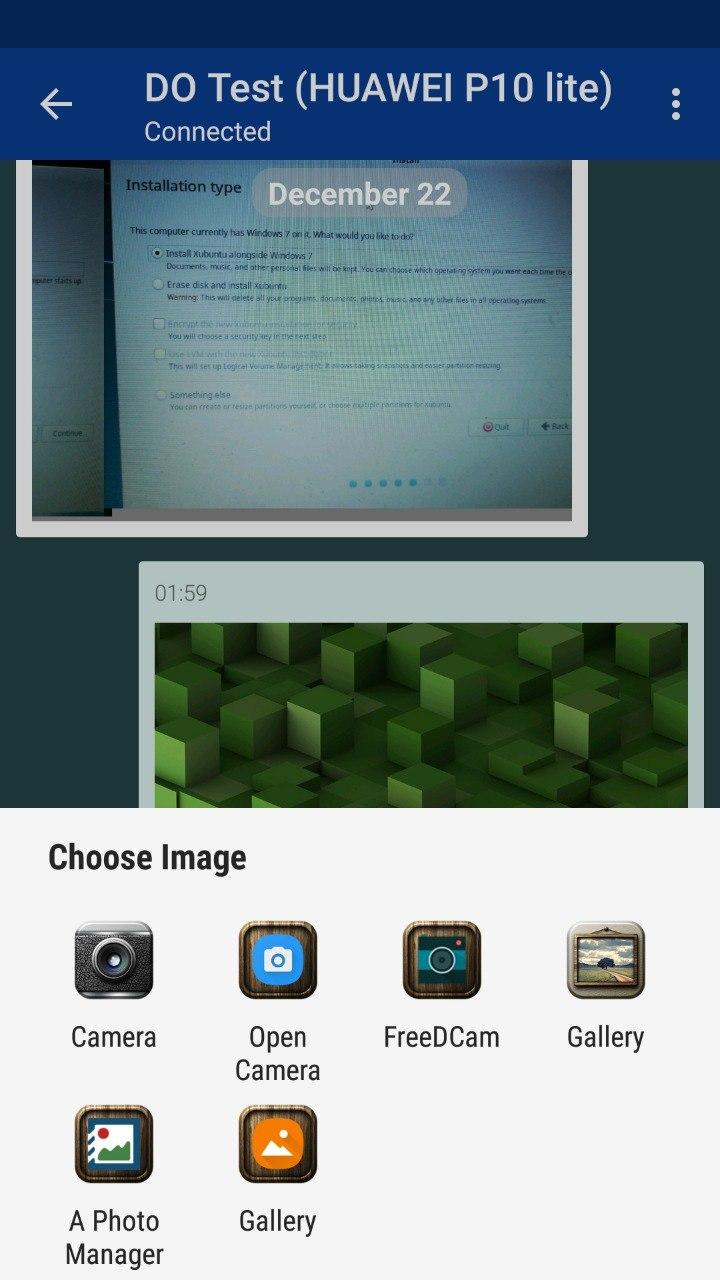
\includegraphics[width=0.8\textwidth]{chat_activity.jpg}
	\caption{Внешний вид экрана чата}
	\label{fig:chat_activity}
\end{figure}

\begin{figure}[ht]
    \centering                                                           
    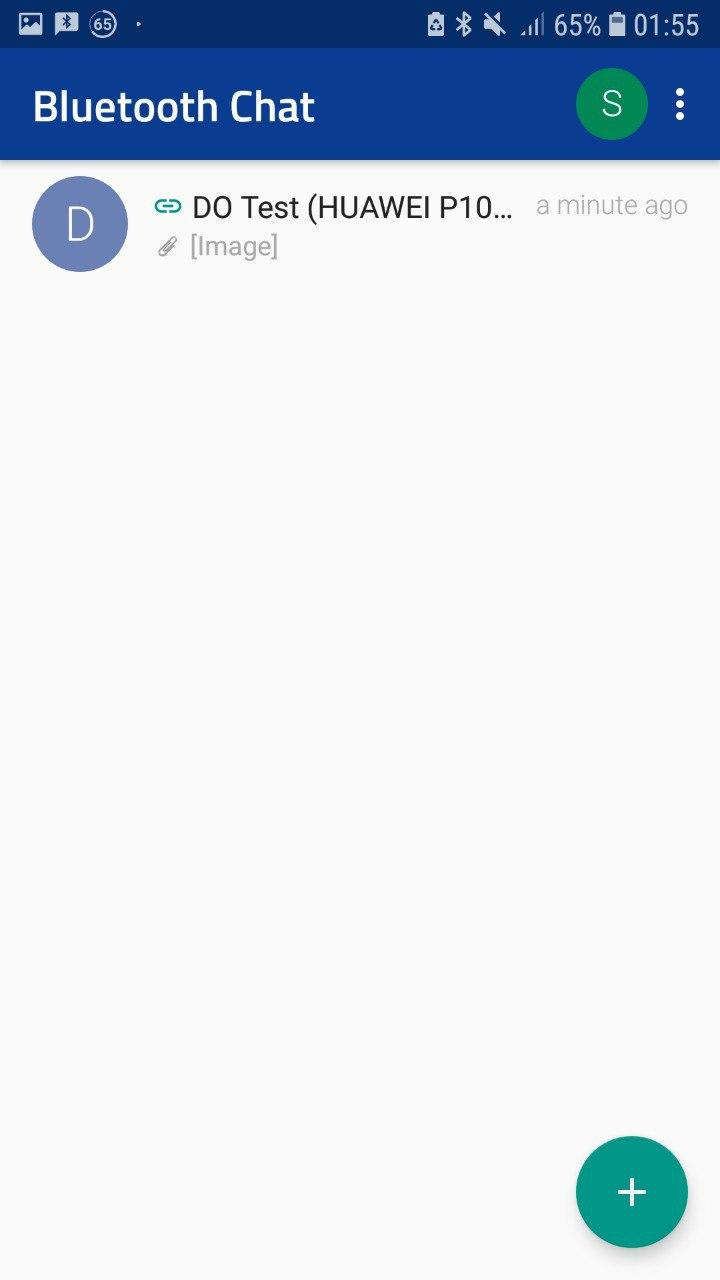
\includegraphics[width=0.8\textwidth]{conversations_activity.jpg}
	\caption{Внешний вид экрана выбора разговора}
	\label{fig:conversations_activity}
\end{figure}

\begin{figure}[ht]
    \centering                                                           
    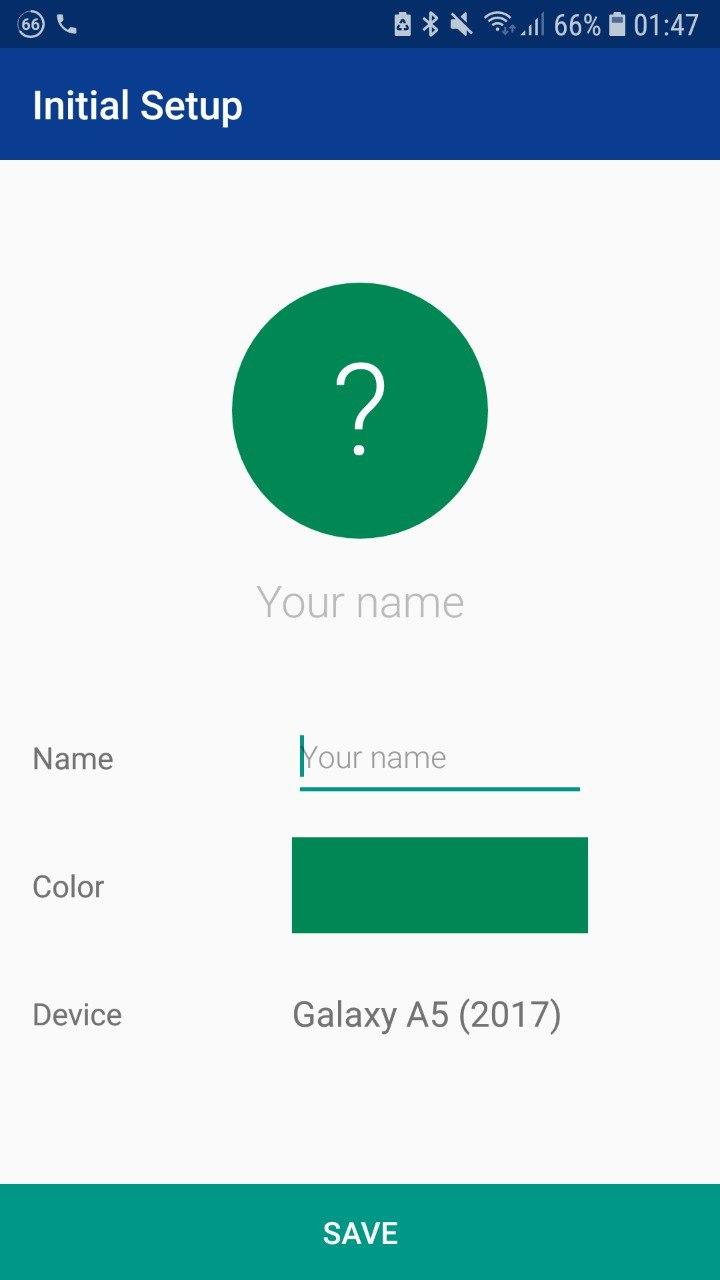
\includegraphics[width=0.8\textwidth]{profile_activity.jpg}
	\caption{Внешний вид экрана профиля}
	\label{fig:profile_activity}
\end{figure}

\begin{figure}[ht]
    \centering                                                           
    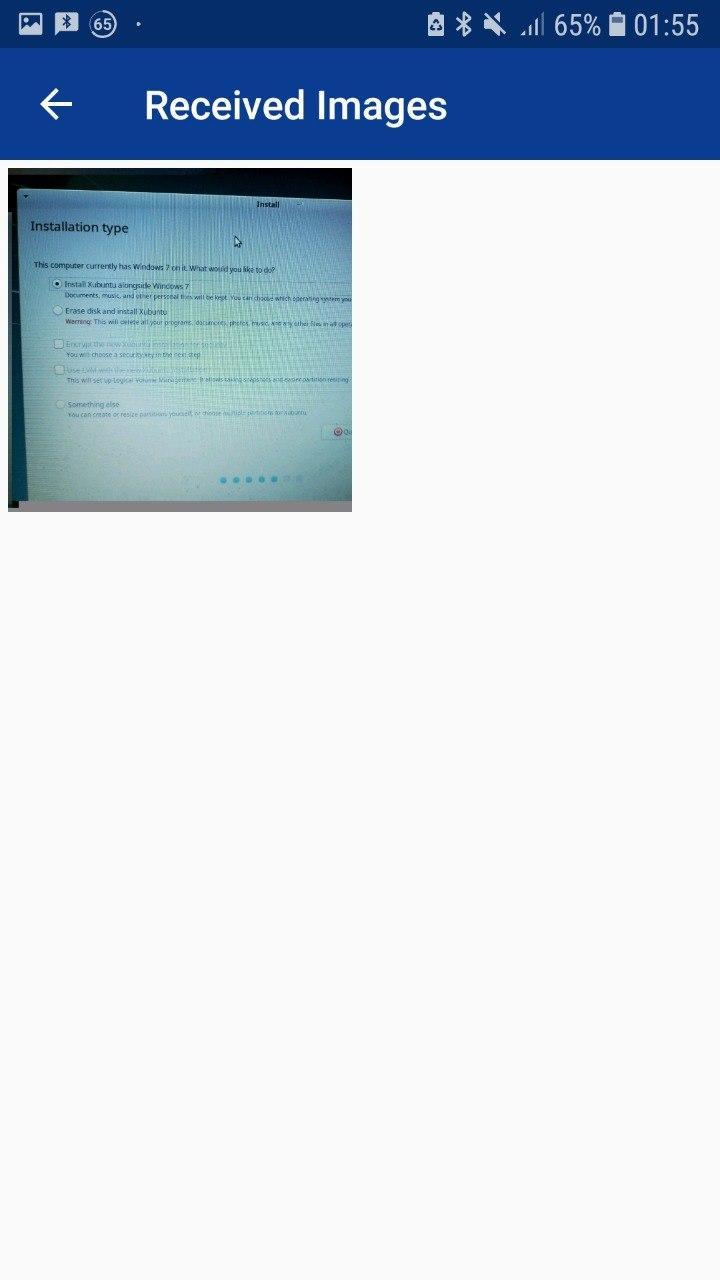
\includegraphics[width=0.8\textwidth]{received_images_activity.jpg}
	\caption{Внешний вид экрана полученный изображений}
	\label{fig:received_images_activity}
\end{figure}

\begin{figure}[ht]
    \centering                                                           
    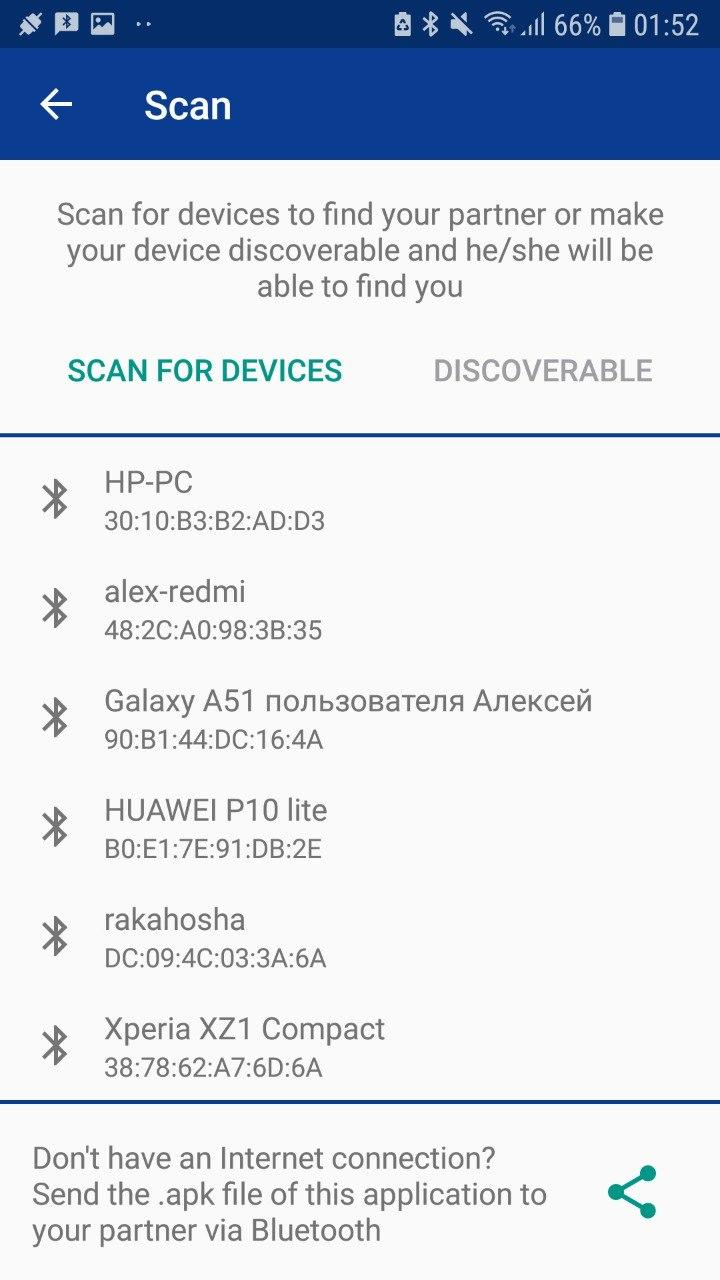
\includegraphics[width=0.8\textwidth]{scan_activity.jpg}
	\caption{Внешний вид экрана сканирования}
	\label{fig:scan_activity}
\end{figure}

\begin{figure}[ht]
    \centering                                                           
    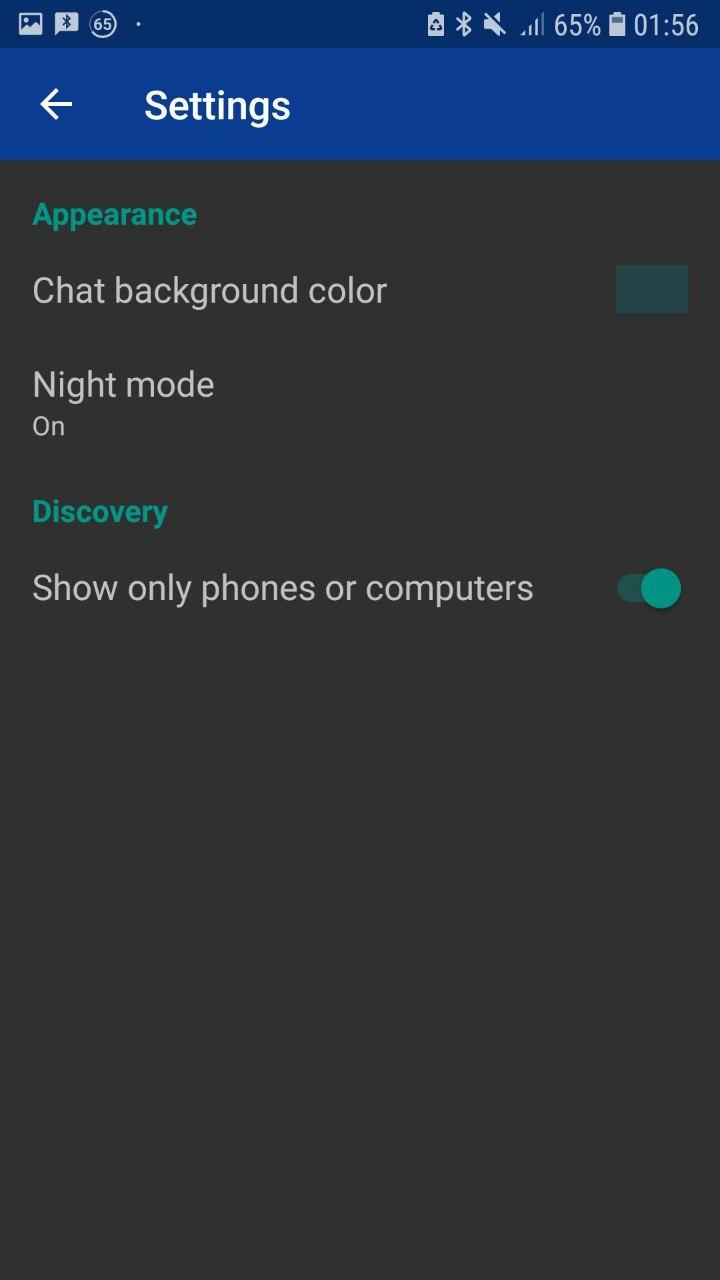
\includegraphics[width=0.8\textwidth]{settings_activity.jpg}
	\caption{Внешний вид экрана настроек}
	\label{fig:settings_activity}
\end{figure}

